\chapter{Projektafgrænsning (JS)}
%afgrænsninger i projektet her.

Et fuldt integreret vandingssystem er, grundet manglende ressourcer og tid, ikke en mulighed på dette semesterprojekt, men der udarbejdes i stedet en skaleret prototype.
Foruden størrelsesbegrænsning er der fra skolens side givet forbud mod, uanset tidligere baggrund, at der arbejdes på 230V, men da der indgår en 230V pumpe i projektet har skolen givet særtilladelse til at der laves et relæ-kredsløb i en lukket kasse, hvori alle ledende dele er helt afskærmet for fysisk kontakt som kan ses på figur \ref{lab:230Vrelay}.

Hurtigt i projektets forløb fik vi tildelt en pumpe fra Grundfos, det viste sig senere at denne ikke kunne bruges til det ønskede formål med at skabe et vandtryk, da denne er en cirkulationspumpe. 

%Løsningen på dette ender med en billig vandpumpe til påmontering på en 230 V %boremaskine. 

\begin{figure}[H]
  \centering
    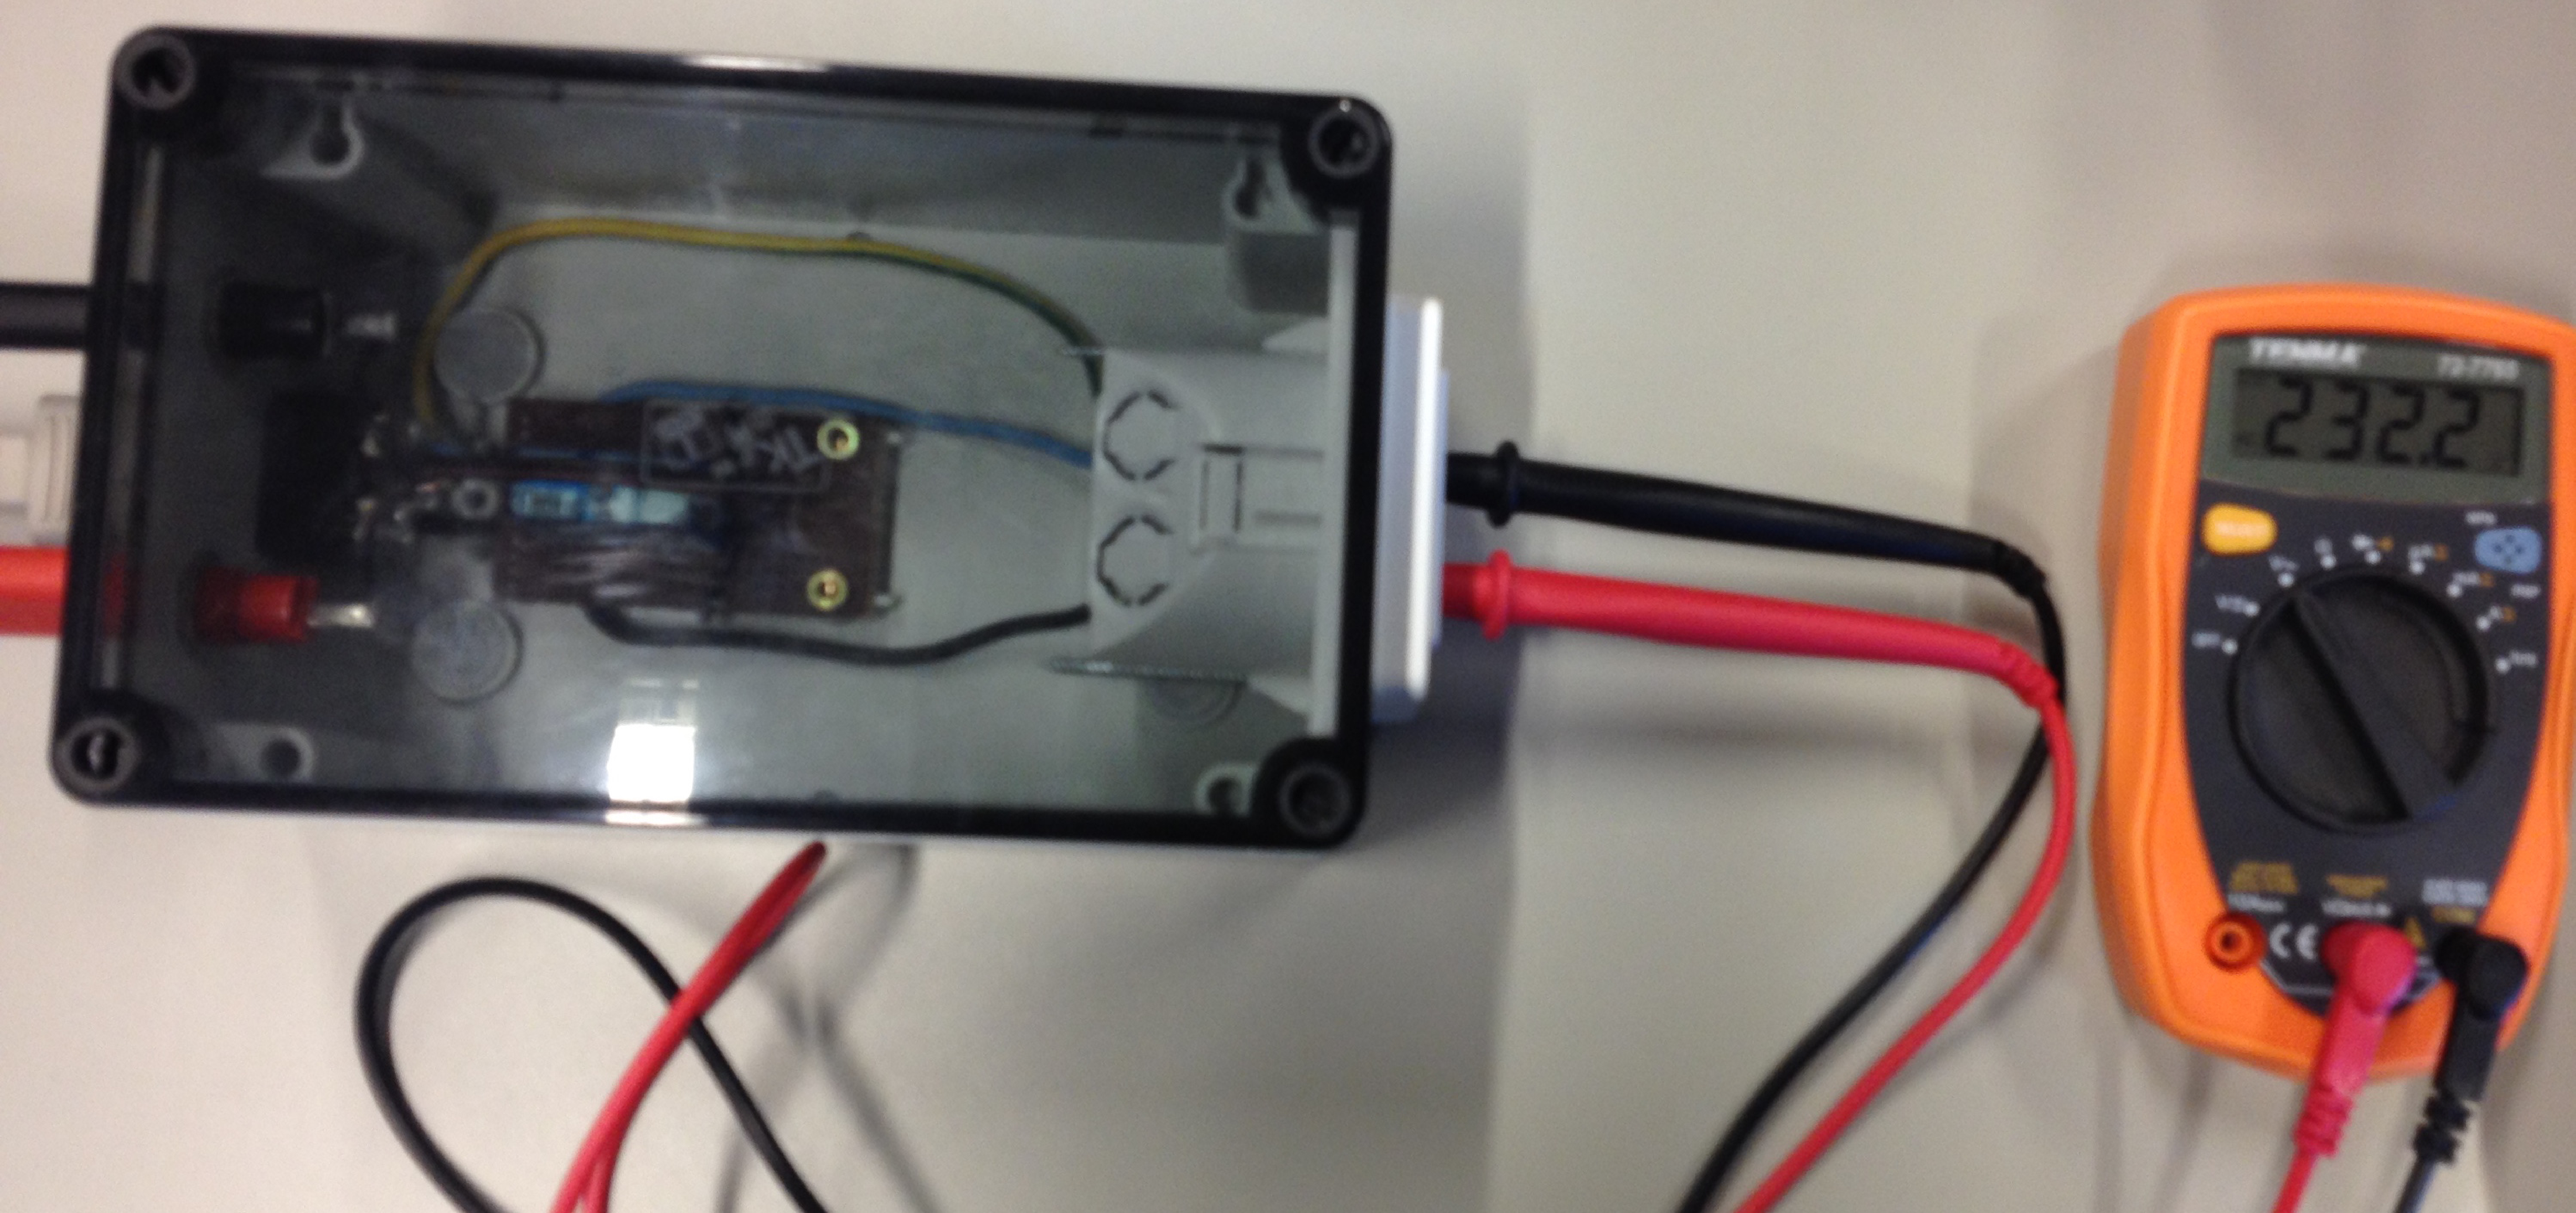
\includegraphics[width=0.75\textwidth]{Billeder/230Vrelay}
    \caption{Relæ i afskærmet kasse}
    \label{lab:230Vrelay}
\end{figure}

Efter at den serielle kommunikation(SPI) var implementeret færdig og klar til test, viste det sig at overførelsesafstanden på 22 cm, som først var tiltænkt, ikke kunne lade sig gøre, da dataen blev korrupt undervejs. Denne afstand blev da nedsat til 7 cm for at kunne overføre data uden fejl.
 

